\pdfminorversion=7
\documentclass[spanish,aspectratio=1610,xcolor={dvipsnames,table}]{beamer}
\geometry{paperwidth=19.2cm,paperheight=12cm}

\usepackage[utf8]{inputenc}
\usepackage[T1]{fontenc}
\usepackage[spanish,es-nodecimaldot]{babel}
\usepackage{lmodern,amsmath,amssymb,booktabs,array,graphicx,ragged2e,tikz,hyperref}
\usetikzlibrary{arrows.meta,positioning,calc,fit,backgrounds}

\newcommand{\studentname}{Mtro. Martín Jonathan de la Cruz Muñoz}
\newcommand{\studentshort}{M. de la Cruz Munoz}
\newcommand{\studentid}{00874}
\newcommand{\studentemail}{martin.delacruz@campus.iiiepe.edu.mx}
\newcommand{\programname}{Maestría en Enseñanza y Aprendizaje de las Matemáticas}
\newcommand{\programshort}{MAEM}
\newcommand{\coursecode}{PFM02}
\newcommand{\coursename}{Temas selectos de matemáticas I}
\newcommand{\courseperiod}{Ago--Nov 2026 (SD26)}
\newcommand{\institutionname}{IIIEPE}
\newcommand{\iiiepelogo}{img/iiiepe/logo-iiiepe-blanco.png}
\newcommand{\iiiepemark}{img/iiiepe/marca-iiiepe.png}

\definecolor{iiiepeNavy}{HTML}{163B5C}
\definecolor{iiiepeBlue}{HTML}{1F6F9F}
\definecolor{iiiepeAqua}{HTML}{20B7A8}
\definecolor{iiiepeOrange}{HTML}{F28C28}
\definecolor{iiiepePaper}{HTML}{F6F8F7}
\definecolor{iiiepeInk}{HTML}{1E2A32}

\mode<presentation>{
  \usetheme{default}
  \usefonttheme{professionalfonts}
  \setbeamertemplate{navigation symbols}{}
  \setbeamertemplate{blocks}[rounded][shadow=false]
}
\hypersetup{colorlinks=true,urlcolor=iiiepeBlue,linkcolor=iiiepeNavy}
\setbeamercolor{background canvas}{bg=white}
\setbeamercolor{normal text}{fg=iiiepeInk,bg=white}
\setbeamercolor{structure}{fg=iiiepeBlue}
\setbeamercolor{frametitle}{fg=white,bg=iiiepeNavy}
\setbeamercolor{title}{fg=white,bg=iiiepeNavy}
\setbeamercolor{block title}{fg=white,bg=iiiepeBlue}
\setbeamercolor{block body}{fg=iiiepeInk,bg=iiiepePaper}
\setbeamercolor{block title alerted}{fg=white,bg=iiiepeOrange}
\setbeamercolor{block body alerted}{fg=iiiepeInk,bg=iiiepeOrange!10}
\setbeamerfont{title}{size=\Large,series=\bfseries}
\setbeamerfont{frametitle}{size=\fontsize{13}{17}\selectfont,series=\bfseries}
\setbeamerfont{block title}{series=\bfseries}
\setbeamertemplate{itemize item}{\textcolor{iiiepeAqua}{$\blacktriangleright$}}

\newcommand{\localLogo}[1]{\IfFileExists{#1}{\includegraphics[height=0.55cm]{#1}}{\textbf{\institutionname}}}
\setbeamertemplate{frametitle}{
  \nointerlineskip
  \begin{beamercolorbox}[wd=\textwidth,ht=1.0cm,dp=0.2cm,leftskip=0.35cm,rightskip=0.25cm]{frametitle}
    \begin{minipage}[c]{0.72\textwidth}\insertframetitle\end{minipage}\hfill\raisebox{-0.08cm}{\localLogo{\iiiepelogo}}
  \end{beamercolorbox}
  \vspace{-0.04cm}{\color{iiiepeOrange}\rule{\textwidth}{1.3pt}}
}
\setbeamertemplate{footline}{
  \leavevmode\hbox{%
    \begin{beamercolorbox}[wd=.34\paperwidth,ht=2.7ex,dp=1ex,leftskip=1em]{author in head/foot}\color{white}\studentshort\end{beamercolorbox}%
    \begin{beamercolorbox}[wd=.42\paperwidth,ht=2.7ex,dp=1ex,center]{title in head/foot}\color{white}\programshort\ -- \coursecode\ (SD26)\end{beamercolorbox}%
    \begin{beamercolorbox}[wd=.24\paperwidth,ht=2.7ex,dp=1ex,rightskip=1em plus 1fil]{date in head/foot}\color{white}Matrícula \studentid\hfill\insertframenumber/\inserttotalframenumber\end{beamercolorbox}%
  }
}
\setbeamercolor{author in head/foot}{bg=iiiepeNavy}
\setbeamercolor{title in head/foot}{bg=iiiepeBlue}
\setbeamercolor{date in head/foot}{bg=iiiepeNavy}

\title{Trabajo Final: Una habilidad, un PDA, cinco minutos}
\subtitle{Actividad 6 (Sesión 13) · Video Didáctico y Modelación en GeoGebra}
\author{\studentname\ (Matrícula \studentid)}
\institute{\institutionname\ · \programname}
\date{14 de noviembre de 2026}

\begin{document}
\begin{frame}[plain]
  \centering
  \vspace{0.5cm}
  \IfFileExists{\iiiepemark}{\includegraphics[height=1.6cm]{\iiiepemark}}{}
  \vspace{0.35cm}
  \begin{beamercolorbox}[sep=10pt,center,rounded=true,wd=0.88\textwidth]{title}
    {\Large\bfseries Trabajo Final: Una habilidad, un PDA, cinco minutos}\\[6pt]
    {\small\color{iiiepePaper} Actividad 6 (Sesión 13) · Video Didáctico y Modelación en GeoGebra}
  \end{beamercolorbox}
  \vspace{0.45cm}
  {\normalsize\bfseries \studentname}\\
  {\small Matrícula \studentid\ · \coursename\ (\coursecode) · \courseperiod}\\
  {\footnotesize 14 de noviembre de 2026}
\end{frame}

\begin{frame}{Trabajo Final: Una Habilidad, un PDA, Cinco Minutos}
  \begin{block}{Estructura Curricular (Sesión 12 $\rightarrow$ Sesión 13)}
    \begin{itemize}
      \item \textbf{Habilidad SEP:} Generalizar relaciones funcionales en sistemas físicos.
      \item \textbf{Contenido:} Variación proporcional directa $F_2 = k\cdot F_1$ con $k = (d_2/d_1)^2$.
      \item \textbf{PDA:} Modela e interpreta $k$ en sistemas hidráulicos validando con tabla y gráfica.
    \end{itemize}
  \end{block}
  \vspace{0.15cm}
  \begin{block}{Producto Audiovisual Generado (StepDeckStudio)}
    Video de \textbf{4:09 min} ($249.08\text{ s}$, $1280\times 720$, $24\text{ fps}$), voz neural española, subtítulos \texttt{.srt} y cumplimiento \textbf{36/36 pts} en la rúbrica de 9 criterios.
  \end{block}
\end{frame}

\begin{frame}{Validación en GeoGebra: Modelo Real vs. Error Frecuente}
  \begin{columns}[T]
    \column{0.58\textwidth}
      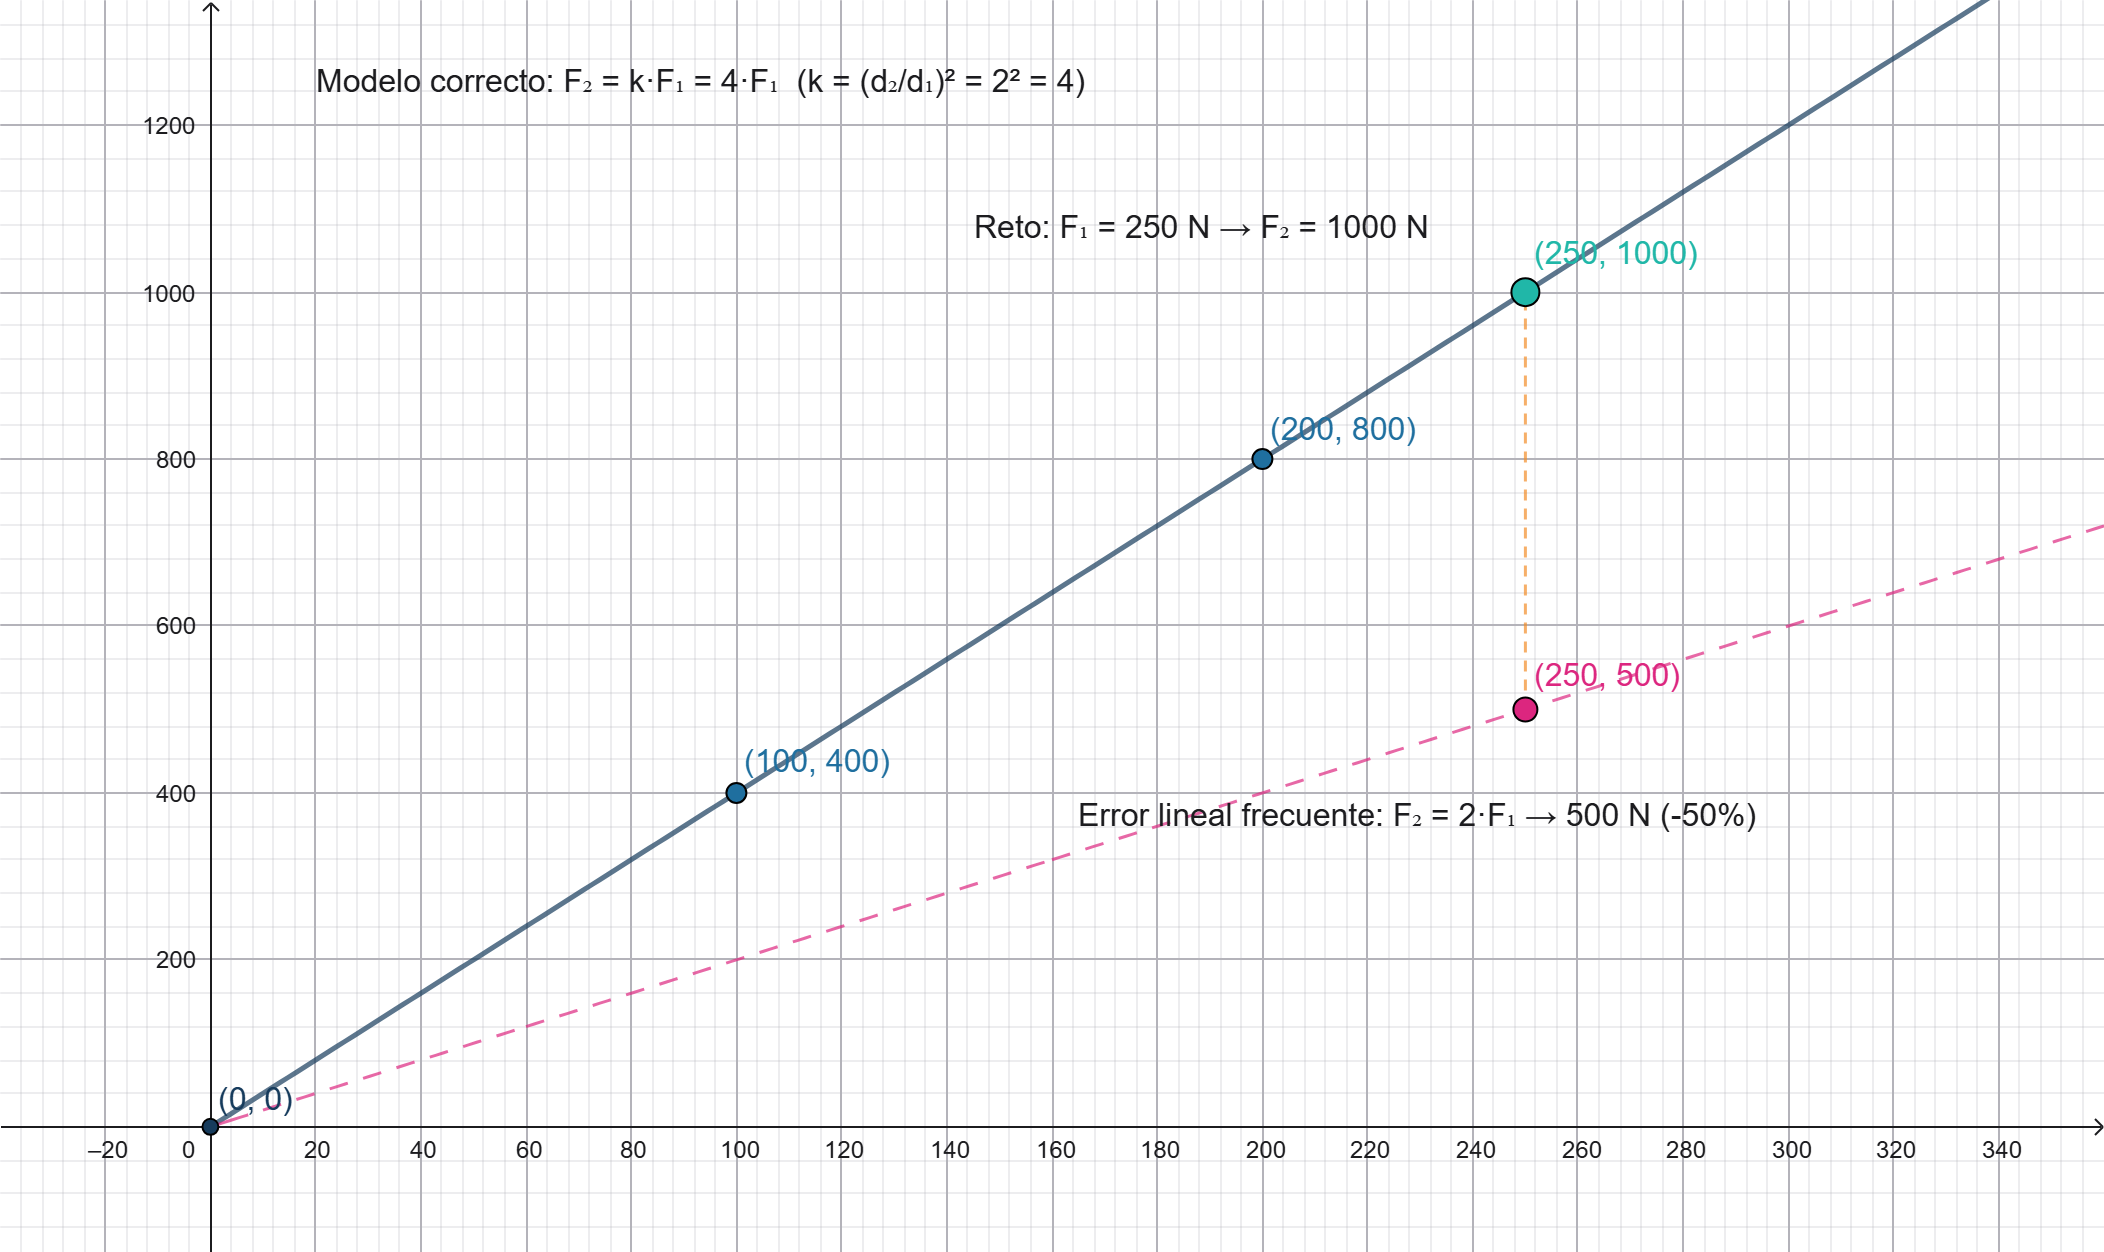
\includegraphics[width=\linewidth]{img/geogebra/act6_proporcionalidad_hidraulica.png}
    \column{0.39\textwidth}
      \begin{block}{Reto de la excavadora}
        Con $d_1=5\text{ cm}$, $d_2=10\text{ cm}$ y $F_1=250\text{ N}$:
        \begin{itemize}
          \item $k = (10/5)^2 = 4 \implies F_2 = 1000\text{ N}$.
          \item Error lineal ($k=2$): $500\text{ N}$ ($-50\,\%$).
          \item Desplazamiento: $\Delta x_2 = 20/4 = 5\text{ cm}$.
        \end{itemize}
      \end{block}
  \end{columns}
\end{frame}

\end{document}
